\documentclass[FIPLY_base.tex]{subfiles}

%\author{Andreas Denkmayr}
%\date{25. Februar 2016}

\begin{document}
\subsection{Advertising mit AdMob}
Mit dem Schalten von Werbung steht eine weitere Einkommensquelle von Apps zur Verfügung.
Es gibt mehrere Dienste die das Schalten von Werbungen unterstützen.
Google AdMob ist der populärste dieser Dienste und wird von Google empfohlen.

\ \\
AdMob unterstützt zwei verschiedene Arten von Werbungen. 
Zum einen gibt es, die sich am Rand des Bildschirms befindlichen, Banner Ads, zum anderen, die den ganzen Bildschirm abdeckenden, Interstitial Ads. \newline
[Google Developers \cite{gdAdMob}]
\ \\
\begin{figure}[h]
	\begin{subfigure}[b]{0.3\textwidth}
	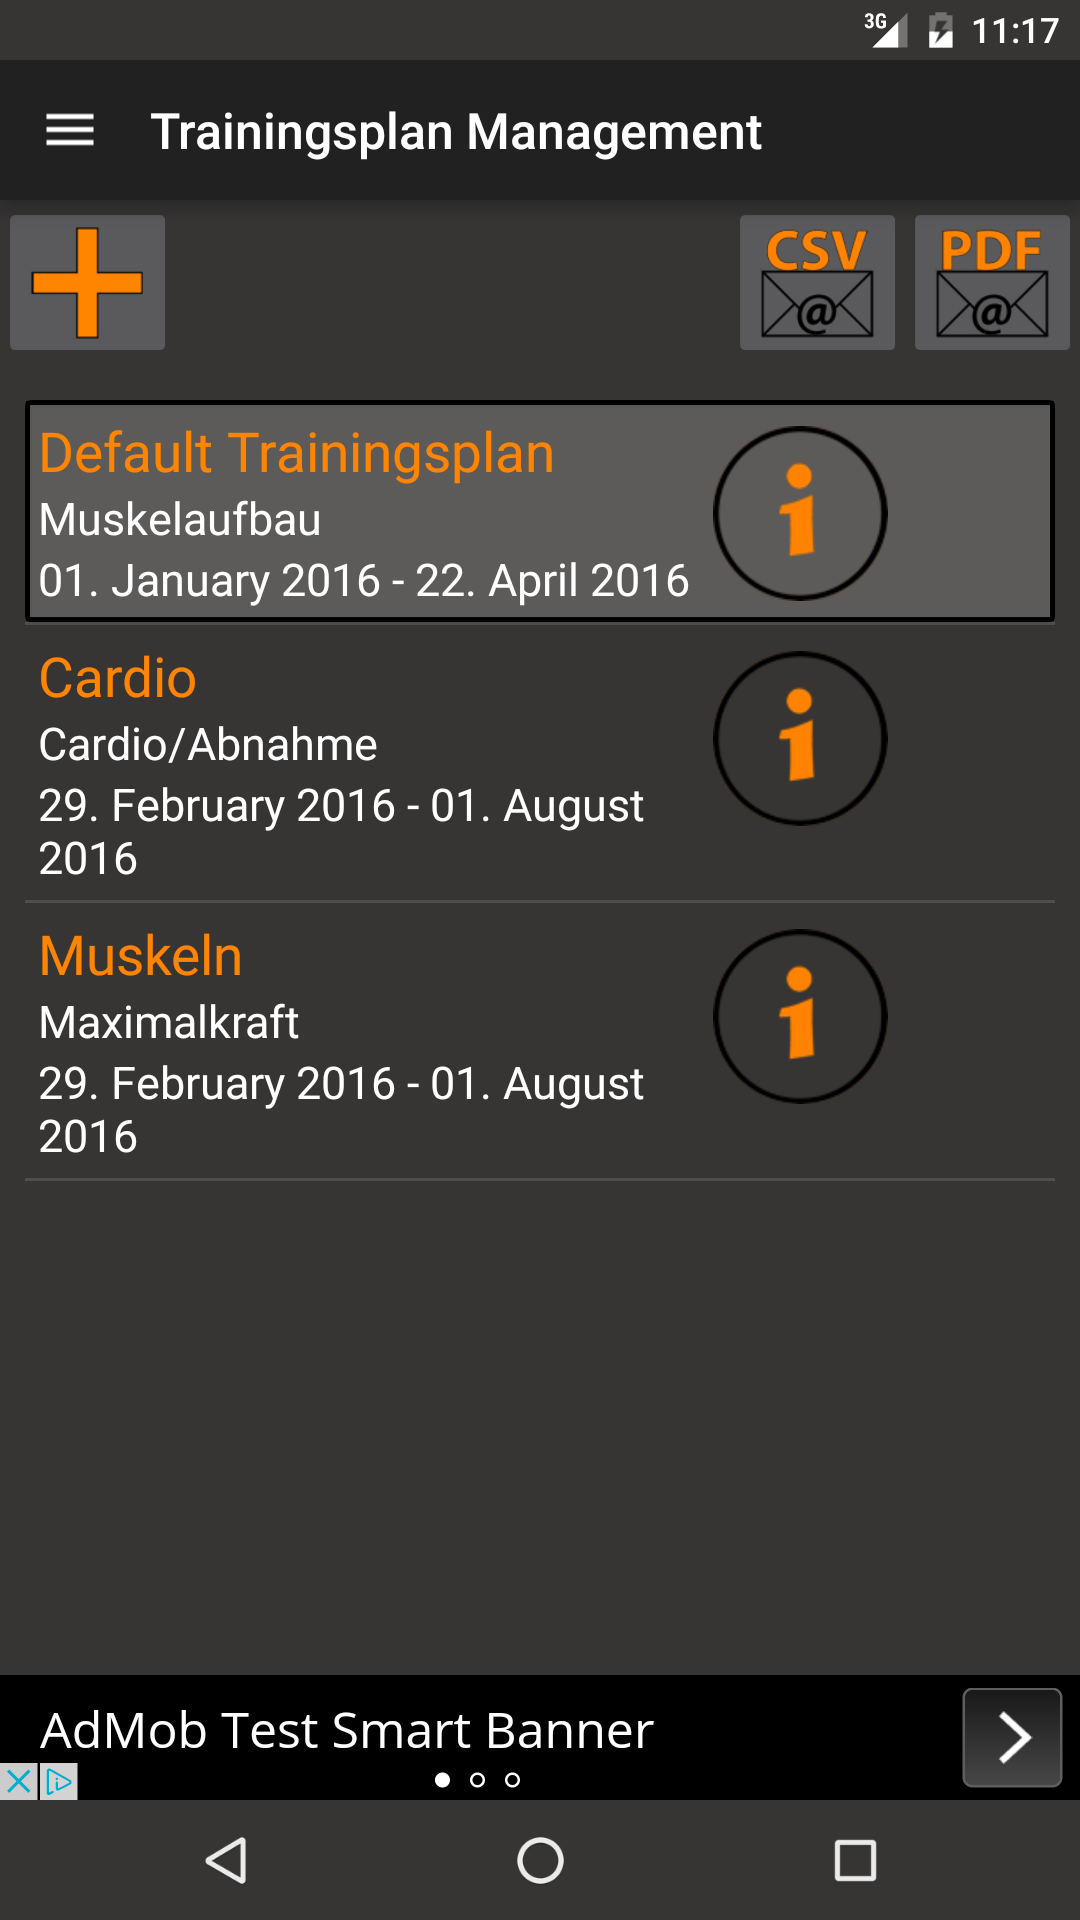
\includegraphics[scale=0.15]{img/adsBanner}
	\end{subfigure}
	\hfil
	\begin{subfigure}[b]{0.3\textwidth}
	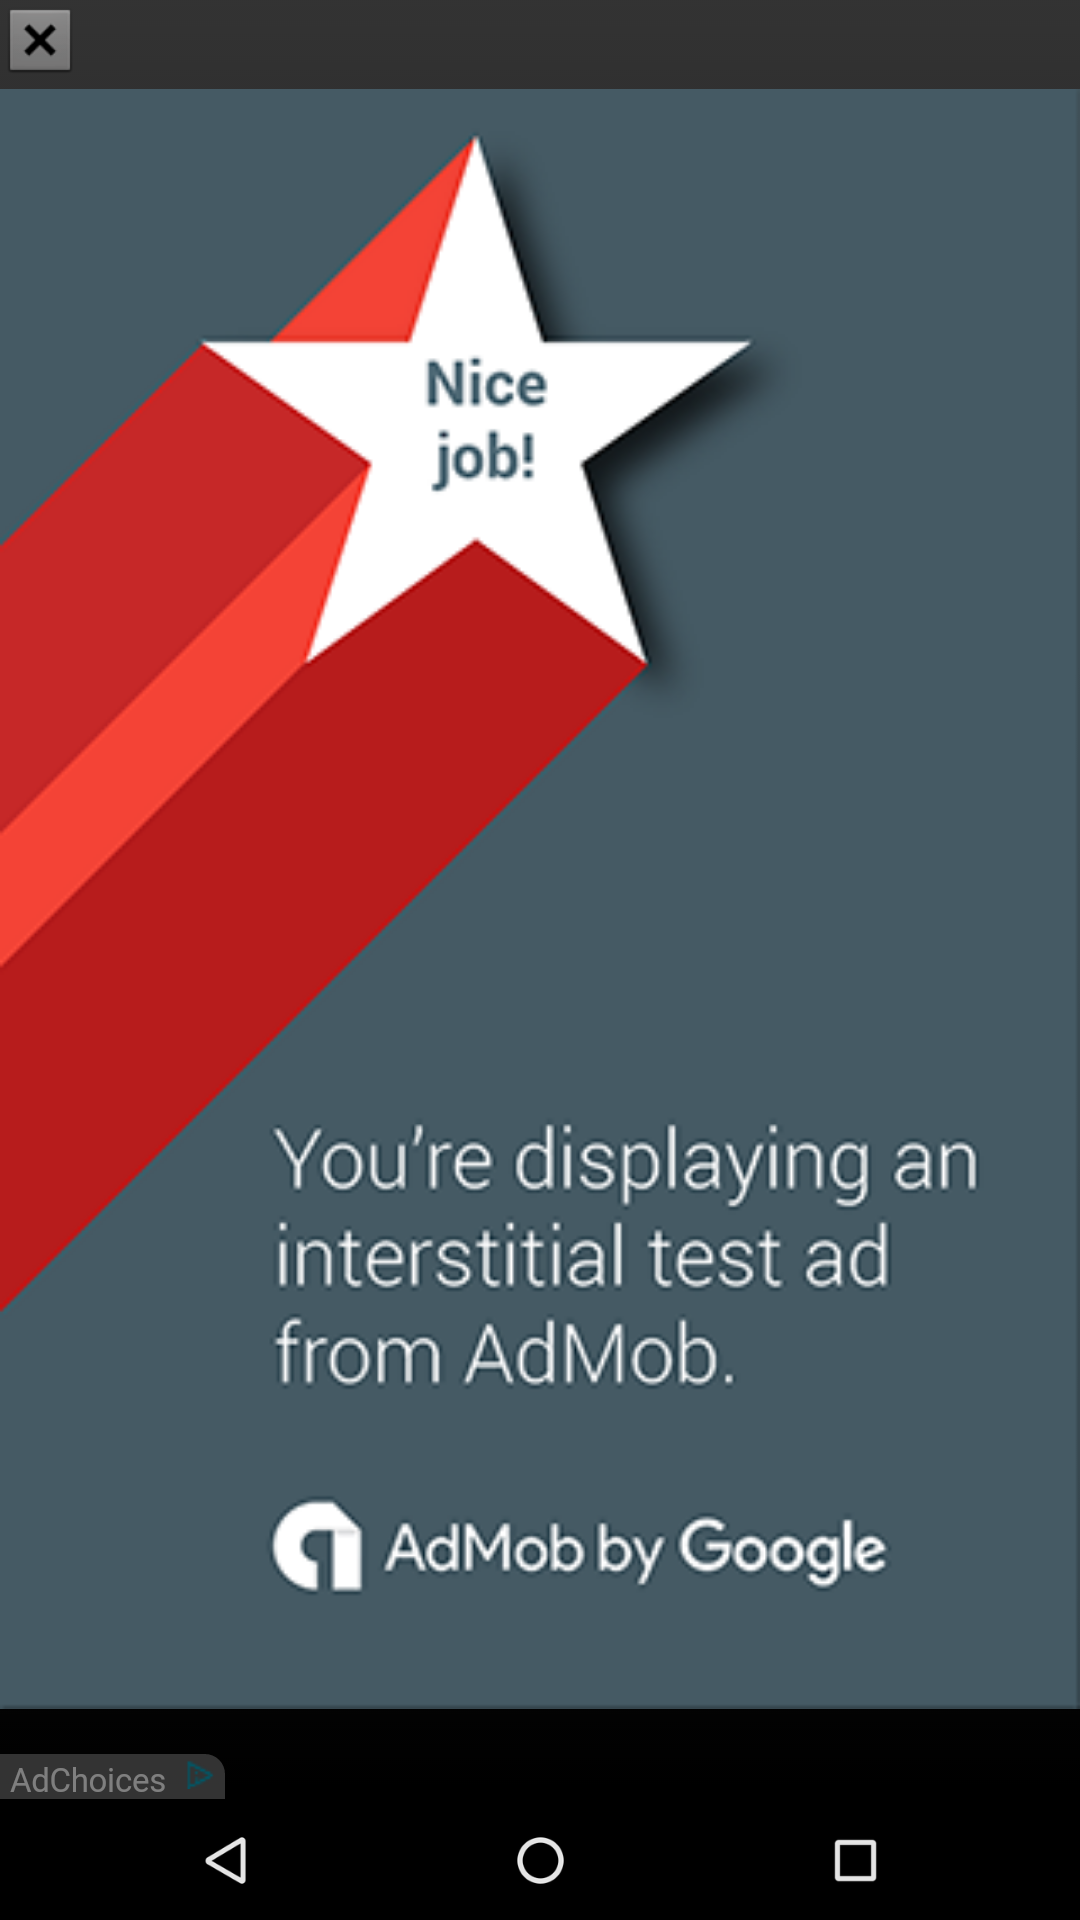
\includegraphics[scale=0.15]{img/adsInterstitial}
	\end{subfigure}
	\caption{Links ist ein Beispiel für eine Banner Ad zu sehen. \newline Rechts sieht man ein Beispiel für ein Interstitial.}
\end{figure}

\newpage
\subsubsection{Banner Ads}
Banner Ads nehmen einen kleinen Teil des Bildschirms ein. Diese werden in einem layout XML file erstellt und dann in einer Activity oder in einem Fragment geladen. Der Benutzer kann durch einen Klick auf das Banner auf die beworbene Webseite weitergeleitet werden. \newline
[Google Developers \cite{gdBanner}]
\ \\
\begin{lstlisting}
<com.google.android.gms.ads.AdView
    android:id="@+id/planAdView"
    android:layout_width="match_parent"
    android:layout_height="wrap_content"
    android:layout_centerHorizontal="true"
    android:layout_alignParentBottom="true"
    ads:adSize="SMART_BANNER"
    ads:adUnitId="ca-app-pub-3940256099942544/1033173712"
    ></com.google.android.gms.ads.AdView>
\end{lstlisting}
Hier wird ein Banner in einem layout XML file definiert. Dieses Banner befindet sich am Boden der App und überspannt die gesamte Breite des Bildschirms.
Die oben eingetragene ad unit Id liefert uns TestAds und dient zum Testen.
\ \\
\begin{lstlisting}
int gender = AdRequest.GENDER_MALE;

AdView mAdView = (AdView) getActivity()
        .findViewById(R.id.planAdView);
AdRequest adRequest = new AdRequest.Builder()
        .addTestDevice(AdRequest.DEVICE_ID_EMULATOR)
        .setGender(gender)
        .build();
mAdView.loadAd(adRequest);
\end{lstlisting}
Dieser Code beinhaltet das Anfordern einer Werbung und anschließend wird das Laden dieser eingeleitet.
Das Banner wird erst dann sichtbar, wenn die Werbung komplett geladen worden ist. 
Die angeforderte Werbung kann durch Daten wie Geschlecht, Geburtstag oder Position präziser auf den Benutzer abgestimmt werden.
Diese Abstimmung erfolgt durch die Methoden .setGender(), .setLocation() und .setBirthday().	

\newpage
\subsubsection{Interstitial Ads}
Interstitial Ads bedecken den gesamten Bildschirm. Wird die Werbung angezeigt, kann der Benutzer die Anzeige schließen oder dem Link der Werbung folgen.
Deshalb eignen sich Interstitials für Apps die gelegentlich zwischen mehreren Bildschirmen wechseln.
Bei diesen Werbungen ist zu beachten, dass die App im Hintergrund weiterläuft, also sollten laute Tonwiedergaben und ressourcenintensive Benutzerinteraktionen pausiert werden. \newline
[Google Developers \cite{gdInterstitials}]
\ \\
\begin{lstlisting}
mInterstitialAd = new InterstitialAd(this);
mInterstitialAd.
       		setAdUnitId("ca-app-pub-3940256099942544/1033173712");
requestNewInterstitial();
\end{lstlisting}
Hier wird eine Interstitial Ad angelegt und anschließend wird eine Werbung für das Interstitial angefordert. 
Die oben eingetragene ad unit Id liefert uns TestAds und dient zum Testen.
\ \\
\begin{lstlisting}
public void requestNewInterstitial() {
        int gender = AdRequest.GENDER_MALE;
        
        AdRequest adRequest = new AdRequest.Builder()
                .addTestDevice(AdRequest.DEVICE_ID_EMULATOR)
                .setGender(gender)
                .build();
        mInterstitialAd.loadAd(adRequest);
    }
\end{lstlisting}
Mit diesem Code wird eine neue Werbung angefordert. Die angeforderte Werbung kann durch Daten wie Geschlecht, Geburtstag oder Position präziser auf den Benutzer abgestimmt werden.
Diese Abstimmung erfolgt durch die Methoden .setGender(), .setLocation() und .setBirthday().	
\ \\
\begin{lstlisting}
if(mInterstitialAd.isLoaded()) 
    mInterstitialAd.show();
\end{lstlisting}
Ist die Werbung geladen kann sie angezeigt werden.\newline
Ebenso sind zahlreiche Methoden im AdListener vorhanden, die es ermöglichen das Verhalten nach einer Interaktion mit der Werbung, zu verwalten.\newline
Deshalb liegt es nahe, die nächste Werbung im onAdClosed() eines AdListeners zu laden, um diese jederzeit auf Abruf anzeigen zu können.

\end{document}
